The aim of this part is to demonstrate the following statement

\begin{thm}
\label{MirThm}
There is a measurable conjugacy $F$ between the earthquake flow $(\lambda , X) \mapsto (\lambda, E_{t \lambda}(X))$ on $\mathcal{ML}\times \mathcal{T}_g $ and the Teichmüller unipotent flow action of \[
u_t = \begin{pmatrix} 1 & t \\ 0 & 1 \end{pmatrix}
\]
on the bundle $\mathcal{QD}$ of nonzero quadratic differentials over Teichmüller space $\mathcal{T}_g$ .
\end{thm}

\[
\xymatrix{
  \mathcal{ML}\times \mathcal{T}_g  \ar[r]^{E_t} \ar[d]_F  & \mathcal{ML}\times \mathcal{T}_g \ar[d]^F \\
   \mathcal{QD} \ar[r]_{u_t} & \mathcal{QD}
 }
\]

To do this we will decompose $F$ between intermediates maps.

\subsection{Tightening map}

A first coresspondance, found by Thurston, exist between measured foliations and measured laminations. We will mostly follow the paper of Levitt \cite{levittfoliations}.

\begin{dfnt}
We say that two foliations are equivalent if we can pass from one to the other by Whithead (see definition below) moves or isotopy (homeomorphism isotopic to the identity).
\end{dfnt}


\begin{dfnt}
Given a measure foliation, an critical segment $\gamma$ is an arc between two singularities along a leaf which is not a simple closed curve.
There is a map $f$ homotopic to the identy that collapse $\gamma$ to a point $x$ and is identity outside a neighboorhood of $\gamma$ which contain no other singularity. Doing so we reduce the number of singularities of the foliation and if the extremities of $\gamma$ are singularities of order $k_1$ and $k_2$, $x$ is now a singularity of the new foliation of order $k_1+k_2-2$.
This action is called a \emph{Whithead move}.
\end{dfnt}


\begin{center}
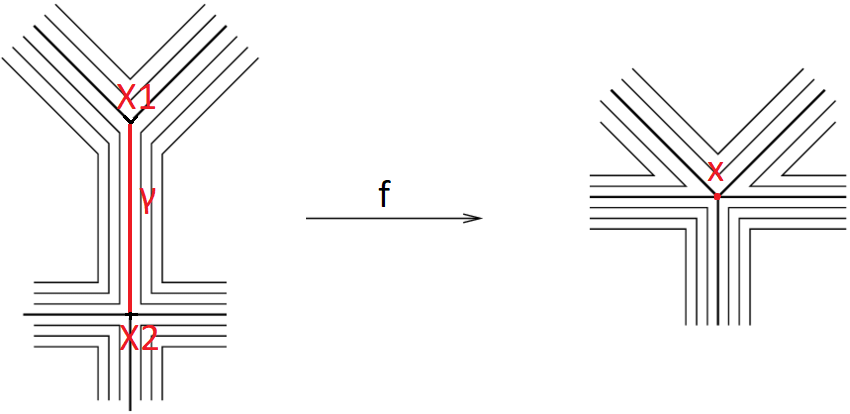
\includegraphics[width=10cm]{Image/Whitehead-move-collapsing-or-creating-an-arc-joining-two-singular-points.png}
\end{center}

\begin{thm}
Let $X$ be a closed orientable hyperbolic surface and $\mathcal{F}$ a foliation. There is a canonical geodesic lamination $\gamma(\mathcal{F})$ associated to $\mathcal{F}$. If $\mathcal{F}$ and $\mathcal{F}'$ are associated foliation then $\gamma(\mathcal{F})= \gamma(\mathcal{F}')$. In the opposite direction given a geodisic lamination $\gamma$, one can find a foliation $\mathcal{F}$ such that $\gamma(\mathcal{F})=\gamma$ and it's unique up to equivalence.
\end{thm}


\begin{dfnt}
A \emph{tranverse curve} is a simple closed curve $C$ which is never tangent to $\mathcal{F}$ and contain no singularity of $\mathcal{F}$.
\end{dfnt}

\begin{rmq}
Since $\mathcal{F}$ contain only saddle singularities, $C$ cannot be contractible, therefor $C$ is isotopic to a simple closed geodesic.
\end{rmq}

We will work on the universal cover of $X$, which is the Poincaré disc $\mathbb{D}$ with circle "at infinity" $\mathbb{S}_{\infty}$. We call $p:X \to \mathbb{D}$ the universal projection.
$\mathcal{\tilde{F}}$ is $p^{-1}(\mathcal{F})$.

We will say that a foliation follow the (*) condition if the following is true:
\begin{center}
If $f_1$ and $f_2$ are two compact homotopic leaves then all leaf in the open annulus between them  is also compact.
\end{center}

\begin{lem}
Let $h$ be a leaf of $\mathcal{\tilde{F}}$. Each end of $h$ converge to a point of $S$; the two point at infinity cannot be the same.
\end{lem}

\begin{proof}
First, we should notice that the behavior of leaf at infinity do not change if we take an equivalent foliation. Indeed a homeomorphism $\phi$ on a compact fundamental domain isotopic to the identy can be extend to an homeomorphism $\tilde{\phi}$ on $\mathbb{D}$ such that $dist(x,\tilde{\phi}(x)) \leq K$. This implie that $\tilde{\phi}$ extend es the identity on the boundary $\mathbb{S}_{\infty}$.

\smallbreak
Then given a leaf $h$ of $\mathcal{\tilde{F}}$, we take a half leah $h_0$. If $p(h_0)$ is compact or spiral toward a compact leaf of $\mathcal{F}$ then the first part of the lemme is imediate.

\smallbreak
Otherwise, $p(h)$ meet a transverse curve $C$ infinitely often. With an isotopie we can take $C$ to be a geodesic. Now $h_0$ can meet a connect component of $\tilde{C}=p^{-1}(C)$ only one time. Otherwise there will be a disk bound by an arc of $\tilde{C}$ and an arc of $h_0$, which is impossible considering the transversity of $C$ and that $\mathcal{F}$ have no $1$-type singularities.

\smallbreak
Now every compact of $\mathbb{D}$ meet a finite number of connected components of $\tilde{C}$ so the limit set of $h_0$ must be on $\mathbb{S}_{\infty}$. This limit set is connected and non empty. Moreover it should not contains any end of a connected component of $\tilde{C}$. But the ends of connected components of $\tilde{C}$ are dense in $\mathbb{S}_{\infty}$ as $\tilde{C}$ is the image of a geodesic by $\pi_1(X)$. This show the first point of the lemma.

\smallbreak
The second assertion is clear if $p(h)$ is compact or if it meet a transverse curve $C$ at least twice since then every connected componnents of $\tilde{C}$ separate the end of $h$.

\smallbreak
Otherwise $p(h)$ spiral toward two compact leaf $f_1$ and $f_2$. If $f_1=f_2$ and the two end point of $h$ are the same then there will be a singularity that would not be a saddle. $f_1 \neq f_2$ is impossible since $\mathcal{F}$ follow the condition (*).
\end{proof}

\smallbreak
We can now associate to every leaf $h$ a geodesic $\gamma(g)$ by joining the endpoint. Then $\tilde{\gamma(\mathcal{F})}= \cup_{h \in \mathcal{F}} \gamma(h)$ is a disjoint union of geodesic invariant by $\pi_1(X)$. We have to show that this set is closed to conclued that we have a lamination.

\begin{lem}
$\tilde{\gamma(\mathcal{F})}$ is closed in $\bar{\mathbb{D}}$
\end{lem}

\begin{proof}

Let $g_n=\gamma(h_n)$ be a sequence of geodesics in $\tilde{\gamma(\mathcal{F})}$ converging to a geodesic $g$. We want to show $g \in \tilde{\gamma(\mathcal{F})}$. We can suppose that all the $g_n$ are distinct of $g$ and are all on the same side.

\smallbreak
Let $L$ be the limit set in $\bar{\mathbb{D}}$. For all leaf $m$ in $\tilde{\mathcal{F}}$, we call $\bar{m}$ the closure of $m$
 by adding the two end point in $\mathbb{S}_{\infty}$. Then $L$ meet at least one connected component of $\bar{\mathbb{D}} \\ \bar{m} $. As the end points of all leaf of $\tilde{\mathcal{F}}$ is a dense subset of $\mathbb{S}_{\infty}$, $L$ contain a leaf $h$. Taking a half-leaf $h_0$, we want to show that the end point is the same as one of $g$.

\smallbreak
A first case is if there is a simple closed curve $C$  transverse to $\mathcal{F}$ which meet $p(h_0)$ infinitely often. If $h_0$ does not converge to the corresponding point at infinity then there would be a connected component of $p^{-1}(C)$ that contains the point of infinity of $h_0$ but does not contain the point of infiny of $h_n$ which is impossible for large $n$.

\smallbreak
A second case is if $p(h_0)$ spirals toward a compact leaf, then closed leaf close to $p(h_0)$ also spirals toward the same compact leaf. Then $h_0$ converges to one of the points at infiniy of $g$ which is a point at inifinity of $h_n$ fot $n$ large.
\smallbreak

Finally if $p(h)$ is compact then $p(h_n)$ spirals toward it for large $n$, therefore $\gamma(h)$ and $g$ have one point in common at infinity. If the second was different, by applying a transformation leaving $\gamma(h)$ invariant (but no $g$), we would separate $h$ from the leaves $h_n$, and it is a contradiction.

\end{proof}

Now we want to exhib an inverse construction which take a lamination $\lambda$ and give a foliation $\mu$. To do this we still consider $\tilde{\lambda}$ in the universal cover. We will suppose that every complementary region is a ideal polygon.
%TODO expliquer pourquoi cette situation est générique

We can built a skeleton that it compose of edge between vertex and a choosen point in the center. After building the skeleton for every polygon we fill the complementary region which will be between four edge by line between the two vertex.

This map is often called the "collapsing" map and its inverse the "tightening" map.
%
\begin{figure}[h!]
\centering
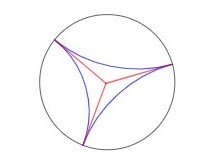
\includegraphics[width=6cm]{Image/CollapsingTightening.jpg}
\caption{In red the skeleton of the ideal triangle in blue, Image from \cite{wright2018mirzakhani}}
\end{figure}

The measure we put on this foliation is uniform on every region between four edges of the skeleton.
%TODO ca semble foireux
\subsection{Correspondance between foliations and quadratic differentials}

For a quadratic differential $q$, one can define two measured foliations, the horizontal $h(q)$ and the vertical $v(q)$ corresponding in locate coordinate to $Re(z)$ and $Im(z)$.

Moreover the measure are \[
h_{\nu} = \int Im(\sqrt{q(z)}dz)
\]
and \[
h{\mu} = \int Re(\sqrt{q(z)}dz)
\]

 This give a map two the pair of foliation but it is not the subjectif, we should restrict to the image.
Define $\Delta = {(\alpha,\beta):i(\alpha,\gamma)=i(\beta,\gamma)=0, \text{ for some }\gamma \in \mathcal{MF}}$. $\Delta$ contain the diagonal $(\alpha,\alpha)$ and is kind of "fat" diagonal.

\begin{lem}
For any $q \in \mathcal{QD}$, $(h(q),v(q)) \notin \Delta$
\end{lem}

\begin{proof}
Suppose that there is $\gamma$ such as $i(h(q),\gamma)=i(v(q),\gamma)=0$ for somme $\gamma \in \mathcal{ML}$. Let take a sequence of simple closed weighted curves $\gamma_i$ converging to $\gamma$. By continuity of the intersection number with have that $i(h(q),\gamma_i) \to 0$. So there is a sequence of saddle connection is the same homotopie class of $\gamma_i$ whose $x$-components is very small. We can have the same argument in the vertical direction and find a contradiction.
\end{proof}

\begin{thm}
The map $q \mapsto (h(q),v(q))$ define a homeomorphism $\mathcal{QD} \to \mathcal{MF} \times \mathcal{MF} \backslash \Delta$
\end{thm}

\begin{proof}
We can describe the inverse map. If we take to measured foliation $h$ and $v$ we can tighten them into lamination (which we also call $h$ and $v$) as in the previous section. This two laminations do not share any leaf, otherwise we would have $(h,v) \in \Delta$ by considering the leaf as a geodesic.
The complementary region of $h \cup v$ are compact polygons, i.e. they do not have a vertex on the boundary of the disk.
Now we can fill the polygon to obtain the quadratic differential with a singularity in each complementary region of order the number of side of the polygon.
\end{proof}

More detail of the proof can be found in \cite{casson_bleiler_1988} Lemma 6.2 and \cite{QuadHub}. The injectivity is discuss with more detail in \cite{Gardiner-1991} section 3.

\subsection{Shear Cordinate}
%NOTE 238 Kerchoff une homotopy sur le disque qui respecte un groupe fushian s'étend sur le bord résultat de Nielsen

Finally there is a map that, given a hyperbolic structure $X$ and a lamination $\lambda$ create a measured foliation which is transverse to $\lambda$.

For simplicity we will ask that $\lambda$ is a maximal lamination i.e. if $\tilde{\lambda}$ is the pre-image of $\lambda$ in the universal cover $\mathbb{D}$, $\mathbb{D}\backslash \tilde{\lambda}$ is made of ideal triangle. We will first work in this triangles minus a region on the center, then give a measure in this foliation, and finnally show that ot is a homeomorphism.

So in one the ideal triangle, given two side we can draw an arc prependicular with the this two sides, which is the intersection of the ideal triangle with the circle tangent to the boundary of $\mathbb{D}$ in the common extremity the two arc chosen. Then by rescaling by a factor $r \in [0;1]$ and doing the same procedure for the two other pair we get a foliation in the ideal triangle minus a locus in the center.


\begin{figure}[h!]
\centering
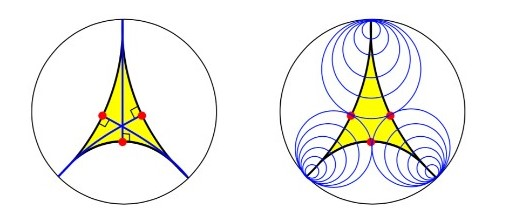
\includegraphics[width=10cm]{Image/FoliationTri.jpg}
\caption{Image from \cite{Martelli2016AnIT}}
\end{figure}

Then we can find a full foliation by pitching the resulting.

We have a natural transverse measure to this foliation. For an arc in one ideal triangle of the lamination we can project it along the leaf of the foliation to asegment in the edge of the ideal triangle, the length of the arc will be the length of the segment. As the leaf are horocycle circle based on the same point, it will not depend of which side we choose to project. Then given an arbitrally arc we decompose it along the ideal triagle it meet.

We want to shwo that this construction is reversable, that is given $\mu \in \mathcal{MF}_\lambda $, the set of foliation transverse to the lamination, we can
construct $X \in \mathcal{T}_g$ whose horocycle foliation is $\mu$.

The idea is that, if we already know $X$, the lamination $\lambda$ can be lift to $\tilde{lambda}$ which is invariant of $\Gamma$ the fushian group of $X$. But we can built $\tilde{lambda}$ only with the information given by $\mu$.

We will note $\tilde{\mu}$ the preimage of $\mu$ in $\mathbb{D}$. If we consider two triangles $T_1$ and $T_2$  that are complementary region of $\tilde{\lambda}$ and we suppose we take a segment $A$ in a leaf of $\tilde{\mu}$ that goes to an edge of $T_1$ to $T_2$. We name $v_1$ and $v_2$ the two vectors with footprint in the edge and tangent to them. Then there is a Moebuis transformation $S$ which take one to the other. With one more information, the "shear", we can place $T_2$ on $\mathbb{D}$, according to the position of $T_1$

\begin{figure}[h!]
\centering
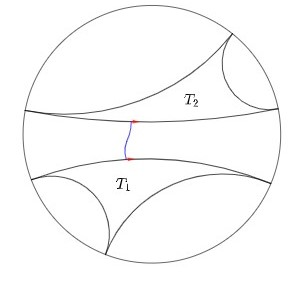
\includegraphics[width=6cm]{Image/Foliation.jpg}
\caption{Image from \cite{wright2018mirzakhani}}
\end{figure}

Indeed given only a Moebuis transformation we still have a one parameter families of triangle $T_2$ with an edge generated by $v_2$. To fix this we trace two orthogeodesic comming from the vertex of the ideal triangles facing the considered edges and from the point of intersection in $T_1$ we follow a leaf of the foliation, then when we meet $T_2$ we have to move along the geodesic edge to find the other point of intersection. This lenght is the shear between $T_1$ and $T_2$

\begin{figure}[h!]
\centering
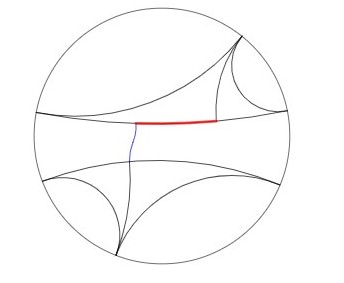
\includegraphics[width=6cm]{Image/Shear.jpg}
\caption{Image from \cite{wright2018mirzakhani}}
\end{figure}

Let $I$ be the set of all triangles in $\mathbb{D}$ that $A$ meet. For each $i\in I$ we can define $v_i^+$ and $v_i^-$ the vectors tangent to the edge of the corresponding triangle at the intersection of the edges and $A$. Note that $I$ is a countable totally ordered but non well ordered set. So if we take $S_i$ the Moebuis transformation which take $v_i^-$ to $v_i^+$, we have to give a meaning of the expression \[
\prod_{i\in I}S_i
\]

\begin{dfnt}
Given a countable totally ordered set of indice $I$ and element $S_i$ in a Banach algebra, we say that $\prod_i S_i$ is \emph{well defined} and equal to $S$ if for any increasing chain \[
I_0 \subset I_1 \subset ... \subset I
\]
with $\cup_k I_k=I$ we have $lim_{k \to \infty} \prod_{i \in I_k}S_i =S $.
\end{dfnt}

\begin{lem}
For element $s_i$ in a Banach algebra index by a countable totallyordered set, if $\sum \| s_i \| < \infty$, then $\prod(1+s_i)$ is well-defined.
\end{lem}
\begin{proof}
For $1 \leq m \leq n$, we have \[
\| \prod_{i=1}^n(1+s_i)-\prod_{i=1,i \neq m}^n (1+s_i) \| \leq \|s_m \| \| \prod_{i=1,i \neq m}^n (1+s_i) \| \leq \|s_m\| \prod_{i=1}^n (1+\|s_i\|)
\]
Or with the assumption $\sum \| s_i \| < \infty$ we have that $\prod(1+\|s_i\|) \leq C < \infty$, so removing or adding $1+s_m$ produce a change bound by $\|s_m\| C$.
\end{proof}

Now we want to apply this lemma to $S_i - Id$, with $Id$ the identity matrice.

\begin{lem}
For the previous $S_i$, if we note $s_i=S_i - Id$ we have $\sum \| s_i \| < \infty$.
\end{lem}

\begin{proof}
Each $S_i$ is conjugate to a horocycle transformation of time one. The conjugacy is made by a geodesic flow along the edges of the triangle. We can compute \[
\begin{pmatrix} e^{-t/2} & 0 \\ 0 & e^{t/2} \end{pmatrix} = \begin{pmatrix} 1 & 1 \\ 0 & 1 \end{pmatrix} \begin{pmatrix} e^{t/2} & 0 \\ 0 & e^{-t/2} \end{pmatrix} = \begin{pmatrix} 1 & 0 \\ 0 & 1 \end{pmatrix}+ \begin{pmatrix} 0 & e^{-t} \\ 0 & 0 \end{pmatrix}
\]
So the norm of $s_i$ is inversally corrolated to the amount of geodesic flow used in the conjugaison.
Now we can parttion the indice set $I$ into finely many subset $(I_k)$ according to to which spike of the lamination the arc of $A$ cross.
Then for a spike the sum of $\|s_i \|$ where $i \in I_k$ is finite, indeed the distance between two neighbooring crossing is bound below by a constant and so the amount of time we should do the geodesic flow increase at most linerally and finnaly the norm of the $s_i$ should decraese geometrically.
\end{proof}

So we can conclude that there is an unique Moebuis transformation $S$ equal to the meaningfull expression $\prod_i S_i$.

Now we can conclude the proof. There exist, without any hyperbolic structure $X$  topological classes for $\tilde{\mu}$ and $\tilde{\lambda}$. We choose one arbitrary ideal triangle $T_1$ in the lamination. For every other triangle $T_2$, the Moeubuis transformation and the shear are data that can be compute only using the transverse measure of $\tilde{mu}$. So we can place $T_2$, and the other triangle. The closure of this set give the lamination $\tilde{\lambda}$. $\tilde{\lambda}$ will be preserve by a fushian group $\Gamma$ and we will have $X=\mathbb{D}  / \Gamma$.

\subsection{Conjugaison between the horocyclic flow and the earthquake flow}

We now have to prove that the map between $\mathcal{ML}\times \mathcal{T}_g $ and $\mathcal{QD}$ conjugate the earthquake flow and the horocyclic flow.

\begin{lem}\label{LemDer}
Denote by $Shear_X(T_1,T_2)$ the shear for two triangles joined by an arc $A$ of the horocyclic foliation on the hyperbolic surface $X$. Then \[
Shear_{E_{t \lambda}(X)}(T_1 ,T_2)= Shear_X(T_1,T_2)+t \lambda(A)
\]
where $\lambda(A)$ denote the transverse measure of $A$ and $t$ is sufficiently small.
\end{lem}

\begin{proof}
$T_1$ and $T_2$ are separeted by infinitely many leaves of $\tilde{\lambda}$. We want to undersant how $T_2$ moved relatively to $T_1$ by the action of the earthquake $E_{t \lambda}$.
We can approximate the measured lamination between the two triangles by a discrete one.
If the earthquake along a leaf of $\gamma$ of $\tilde{\lambda}$ between $T_1$ and $T_2$ by an amount $t$, then this changes the shear coordinate between $T_1$ and $T_2$ by $t$. Indeed each arc of the horocycle foliation which have endpoint on $\gamma$ see their endpoints translated by $t$.
Similary if the earthquake moves finitelymany leave of $\lambda$ with measure $a_i$, the shear changes by precisely $t \sum a_i$. So taking a limit, we have the lemma for an arbitrary measured foliation.
\end{proof}

We will now show that the Mirzakhani's map conjugates the earthquake flow to the horocyclic flow. Let $\mathcal{ML}_0$ denote the set of maximal lamination and $\mathcal{QD}_0$ the locus of quadratic differentials with simple zeros and no horizontal saddle connection. We begin with an easy lemma.

\begin{lem}
An arc joining two singularities of a quadratic differential have in is isotopy class a path made of horizontal and vertical arc between two singularities of the quadratic differential.
\end{lem}

\begin{cor}
Suppose$q_t$ is a path in the space of quadratic differential such that for every $t_0$ and every path $\gamma$ on $q_{t_0}$ joining two singularities, the period $x_t + i y_t$ of $\gamma$ satisfied \[
\frac{d}{dt}|_{t=t_0} x_t = y_{t_0}, \frac{d}{dt}|_{t=t_0} y_t = 0
\]
Then $q_t$ is an orbit of the horocyclic flow.
\end{cor}

\begin{proof}
We have \[
\begin{pmatrix} 1 & t \\ 0 & 1 \end{pmatrix} \begin{pmatrix} x \\ y \end{pmatrix} = \begin{pmatrix} x + t y \\ y \end{pmatrix}
\]
And we can integrate the two equations to find the linear action.
\end{proof}

We can now prove theorem \ref{MirThm}.

\begin{proof}
We want to show that \[
q(\lambda,F_{\lambda}(E_{t \lambda}(X)))
\]
%TODO vérifier que ces fonctions ont des noms
is a horocyclic flow path. We pick an arbitrary time $t_0$ and look at the derivative of the path, called $\gamma$. The coordinate $y_t$ is constant equal to $\lambda(\gamma)$ and the derivative of $x_t$ is by lemma\ref{LemDer} equal to $y_t$. We conclude by the previous lemma.
\end{proof}
